\definecolor{accsblue}{RGB}{15,77,146}
\definecolor{coptred}{RGB}{182,67,66}
\definecolor{crcgreen}{RGB}{66,148,158}
\definecolor{globalgray}{RGB}{150,150,150}
\definecolor{targetgray}{RGB}{110,110,110}

\pgfplotsset{
  paperaxis/.style={
    tick label style={font=\small},
    label style={font=\small},
    title style={font=\normalsize, align=left},
    legend style={font=\small, draw=none, fill=none},
    axis line style={black, line width=0.7pt},
    tick style={black, line width=0.6pt},
    major grid style={draw=none},
    every axis plot/.append style={line width=0.9pt},
  }
}

\newcommand{\FigureSelectionAmplificationTikZ}{%
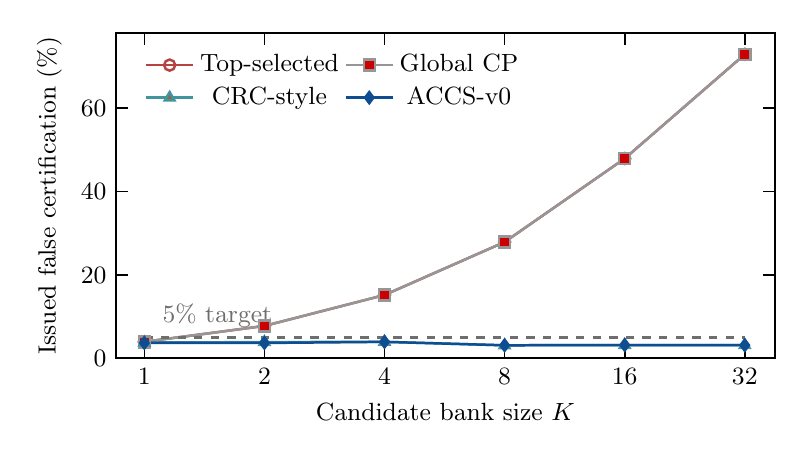
\begin{tikzpicture}
\begin{axis}[
  paperaxis,
  width=0.82\textwidth,
  height=2.25in,
  xmode=log,
  log basis x=2,
  xmin=0.85,
  xmax=38,
  ymin=0,
  ymax=78,
  xtick={1,2,4,8,16,32},
  xticklabels={1,2,4,8,16,32},
  ytick={0,20,40,60},
  xlabel={Candidate bank size $K$},
  ylabel={Issued false certification (\%)},
  legend columns=2,
  legend pos=north west,
]
\addplot+[mark=o, color=coptred] coordinates {
  (1,3.99) (2,7.79) (4,15.20) (8,27.90) (16,47.91) (32,72.88)
};
\addlegendentry{Top-selected}
\addplot+[mark=square*, color=globalgray] coordinates {
  (1,3.99) (2,7.79) (4,15.20) (8,27.90) (16,47.91) (32,72.88)
};
\addlegendentry{Global CP}
\addplot+[mark=triangle*, color=crcgreen] coordinates {
  (1,3.81) (2,3.92) (4,3.98) (8,3.15) (16,3.22) (32,3.17)
};
\addlegendentry{CRC-style}
\addplot+[mark=diamond*, color=accsblue] coordinates {
  (1,3.72) (2,3.71) (4,3.98) (8,3.15) (16,3.22) (32,3.17)
};
\addlegendentry{ACCS-v0}
\addplot[dashed, color=targetgray] coordinates {(1,5) (32,5)};
\node[anchor=south west, font=\small, text=targetgray] at (axis cs:1.05,5) {5\% target};
\end{axis}
\end{tikzpicture}%
}

\newcommand{\FigureAuditLayersTikZ}{%
\begin{minipage}[t]{0.48\textwidth}
\centering
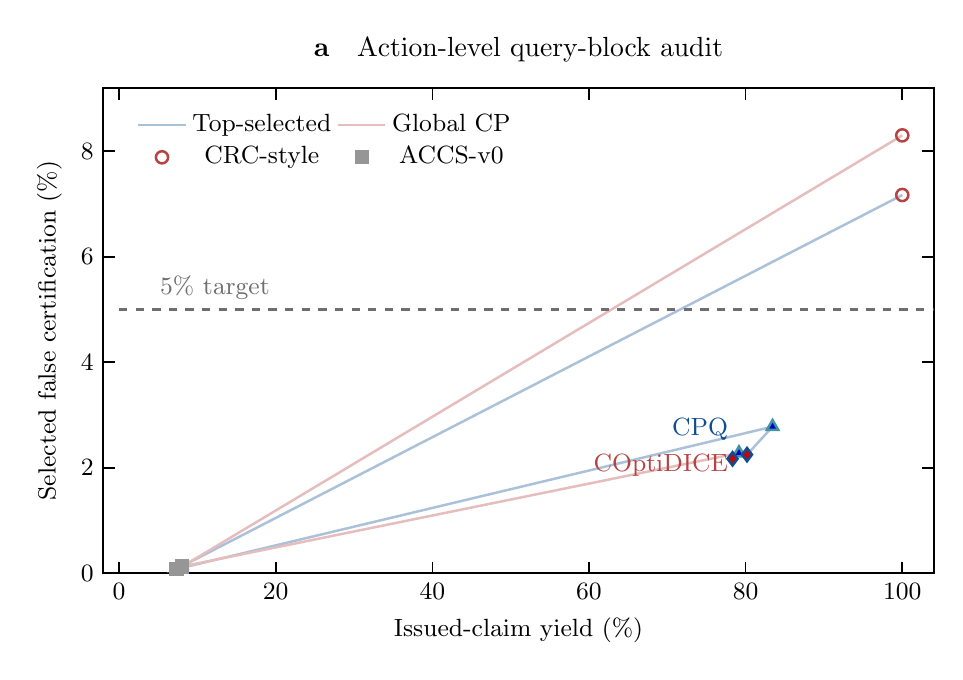
\begin{tikzpicture}
\begin{axis}[
  paperaxis,
  width=\linewidth,
  height=3.05in,
  xmin=-2,
  xmax=104,
  ymin=0,
  ymax=9.2,
  xtick={0,20,40,60,80,100},
  ytick={0,2,4,6,8},
  xlabel={Issued-claim yield (\%)},
  ylabel={Selected false certification (\%)},
  title={\textbf{a}\quad Action-level query-block audit},
  legend columns=2,
  legend pos=north west,
]
\addplot[color=accsblue!35] coordinates {(100,7.17) (7.33,0.08) (83.44,2.78) (80.18,2.25)};
\addplot[color=coptred!35] coordinates {(100,8.30) (8.08,0.13) (79.15,2.28) (78.33,2.17)};
\addplot+[only marks, mark=o, mark size=2.2pt, color=coptred] coordinates {(100,7.17) (100,8.30)};
\addlegendentry{Top-selected}
\addplot+[only marks, mark=square*, mark size=2.1pt, color=globalgray] coordinates {(7.33,0.08) (8.08,0.13)};
\addlegendentry{Global CP}
\addplot+[only marks, mark=triangle*, mark size=2.4pt, color=crcgreen] coordinates {(83.44,2.78) (79.15,2.28)};
\addlegendentry{CRC-style}
\addplot+[only marks, mark=diamond*, mark size=2.4pt, color=accsblue] coordinates {(80.18,2.25) (78.33,2.17)};
\addlegendentry{ACCS-v0}
\addplot[dashed, color=targetgray] coordinates {(0,5) (104,5)};
\node[anchor=south west, font=\small, text=targetgray] at (axis cs:4,5) {5\% target};
\node[anchor=east, font=\small, text=accsblue] at (axis cs:79.0,2.72) {CPQ};
\node[anchor=east, font=\small, text=coptred] at (axis cs:79.0,2.05) {COptiDICE};
\end{axis}
\end{tikzpicture}
\end{minipage}\hfill
\begin{minipage}[t]{0.48\textwidth}
\centering
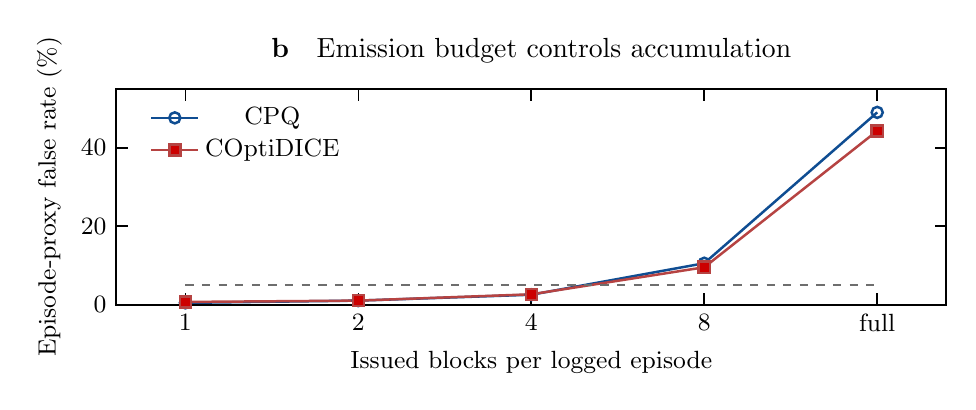
\begin{tikzpicture}
\begin{axis}[
  paperaxis,
  width=\linewidth,
  height=1.7in,
  ymin=0,
  ymax=55,
  symbolic x coords={1,2,4,8,full},
  xtick=data,
  xlabel={Issued blocks per logged episode},
  ylabel={Episode-proxy false rate (\%)},
  title={\textbf{b}\quad Emission budget controls accumulation},
  legend pos=north west,
]
\addplot+[mark=o, color=accsblue] coordinates {(1,0.46) (2,1.03) (4,2.53) (8,10.57) (full,49.08)};
\addlegendentry{CPQ}
\addplot+[mark=square*, color=coptred] coordinates {(1,0.69) (2,1.03) (4,2.64) (8,9.54) (full,44.37)};
\addlegendentry{COptiDICE}
\addplot[dashed, color=targetgray] coordinates {(1,5) (full,5)};
\end{axis}
\end{tikzpicture}

\vspace{0.18in}
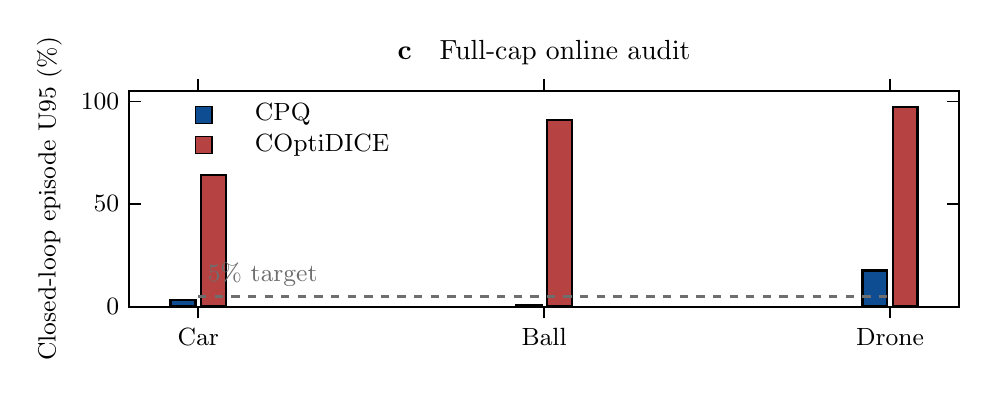
\begin{tikzpicture}
\begin{axis}[
  paperaxis,
  width=\linewidth,
  height=1.7in,
  ybar,
  bar width=9pt,
  ymin=0,
  ymax=105,
  symbolic x coords={Car,Ball,Drone},
  xtick=data,
  ylabel={Closed-loop episode U95 (\%)},
  title={\textbf{c}\quad Full-cap online audit},
]
\addplot+[fill=accsblue, draw=black] coordinates {(Car,3.22) (Ball,0.50) (Drone,17.61)};
\addplot+[fill=coptred, draw=black] coordinates {(Car,64.15) (Ball,90.89) (Drone,97.23)};
\addplot[dashed, color=targetgray, sharp plot] coordinates {(Car,5) (Drone,5)};
\node[anchor=south west, font=\small, text=targetgray] at (axis cs:Car,5) {5\% target};
\node[draw=black, fill=accsblue, minimum width=6pt, minimum height=6pt, inner sep=0pt] at (rel axis cs:0.09,0.89) {};
\node[anchor=west, font=\small] at (rel axis cs:0.14,0.89) {CPQ};
\node[draw=black, fill=coptred, minimum width=6pt, minimum height=6pt, inner sep=0pt] at (rel axis cs:0.09,0.75) {};
\node[anchor=west, font=\small] at (rel axis cs:0.14,0.75) {COptiDICE};
\end{axis}
\end{tikzpicture}
\end{minipage}%
}
